\section{实验评估}
\label{sec:exp_imitation}
本节提供实验以评估 DIDA 在广泛任务中的表现。
首先在\Cref{subsec:setting_exp_imitation} 中描述实验设置，然后在\Cref{subsec:results_imitation} 中展示并讨论结果。



\subsection{实验设置}
\label{subsec:setting_exp_imitation}

除 Trading 任务外，对所有任务运行 DIDA 和基线方法，取 10 个种子的结果进行平均。
Trading 任务的详细说明如下。

\subsubsection{任务}
\label{subsubsec:tasks_imitation}

\noindent\textbf{Pendulum。}\indent 与前一章相同，采用 Pendulum 环境，因其对延迟敏感。
考虑 $\{3, 5, 10, 15, 20\}$ 中的常值延迟。
对该任务，执行 500 个 epoch，每个 epoch 5,000 步，总计 250 万步。

\noindent\textbf{随机 Pendulum。}\indent 引入前一章定义的 Pendulum 随机版本，以评估 DIDA 在随机环境中的表现。
考虑常值延迟 5，执行 500 个 epoch，每个 epoch 5,000 步，总计 250 万步。

\noindent\textbf{非整数延迟 Pendulum。}\indent 为测试 DIDA 在非整数延迟上的表现，提出以下设置。
首先，学习一个持久度（persistence）为 2 的无延迟专家，其中持久度表示智能体在选择新动作之前重复执行同一动作的次数~\cite{metelli2020control}。
本质上，持久度为 2 时，智能体的控制频率减半。
DIDA 将在时间步集合 $(2t)_{t\in\naturalnumbers}$（与专家相同）中的状态下执行，而 DIDA 观测到的状态的时间步在 $(2t+1)_{t\in\naturalnumbers}$ 中。

\noindent\textbf{Mujoco。}\indent 类似地，引入四个 mujoco 环境：Walker2d、HalfCheetah、Reacher 和 Swimmer。
对这些任务，考虑常值延迟 5，执行 1,000 个 epoch，每个 epoch 5,000 步，总计 500 万步。

\noindent\textbf{Trading。}\indent 在该任务中，智能体以 10 分钟的控制频率交易 EUR-USD（\texteuro/\$）货币对，涵盖 2016-2019 年期间。
遵循 \cite{bisi2020foreign} 和 \cite{riva2021learning} 的框架，智能体相对于固定金额的 USD 可以选择买入（buy）、卖出（sell）或持平（flat）。
不考虑交易费用；但考虑买卖价差，其对奖励的影响在实践中等同于交易费用。
在该框架中，考虑 50 秒的常值动作执行延迟。
这导致非整数延迟。
在该任务中，使用 2016-2017 年数据训练不同方法，2018 年数据验证超参数，2019 年数据测试。
需要验证集是因为数据集由历史数据构成；
该任务是批量强化学习（batch \gls{rl}）或离线强化学习（offline \gls{rl}）任务，方法可能对训练集过拟合。

\noindent\textbf{同时学习多重延迟。}\indent 对于 Pendulum 和 mujoco 环境，同时评估 DIDA 在较大延迟上训练、在较小延迟上测试时的表现。
考虑在延迟 10 上训练 DIDA，然后在 $[\![1,9]\!]$ 的较小延迟上测试 Pendulum；类似地，在 mujoco 任务中，训练延迟为 5。


\subsubsection{基线方法}
考虑\Cref{subsubsec:baselines} 中使用的基线方法，采用相同超参数。
这些基线方法包括：无记忆 \gls{trpo}（M-TRPO）、增广状态 \gls{trpo}（A-TRPO）、增广状态 \gls{sac}（A-SAC）、无记忆 \gls{sac}（M-SAC）、SARSA 和 dSARSA（$\lambda=0.9$）。
同时包含之前的方法 L2-TRPO 和 D-TRPO。

同时考虑 M-DIDA（见\Cref{subsubsec:dida_no_undelayed_env}）作为基线，以评估是否需要访问无延迟环境。

对于 Trading 任务，用于训练 DIDA 的无延迟专家通过 2018 年的超参数验证选出。
也可以在延迟数据集上对 2018 年的超参数进行验证，以选择一个在延迟上泛化能力更强的专家（尽管是在无延迟数据上训练的）。
在实验中将此基线称为"延迟专家"（delayed expert）。

对于 Pendulum，还包含 BC-DIDA，对应于 DIDA 但使用行为克隆（behavioral cloning）~\cite{bain1995framework} 替代 \textsc{DAgger} 作为模仿算法。
该基线用于研究模仿算法选择的影响。


\subsubsection{DIDA 设置}
\label{subsubsection:our_approach_dida}
在所有实验中，为与其他基线进行公平的样本效率比较，将训练无延迟专家所需的步数纳入考虑，并相应平移 DIDA 的起始样本数。
在图中以垂直虚线表示。
关于无延迟专家本身，从前述理论可见，更平滑的专家对模仿延迟策略的性能界有利（\Cref{th:perf_diff_bound}）。
因此，除 Trading 任务外，所有实验均采用 \gls{sac} 作为专家。
关于平滑策略的研究~\cite{mysore2021regularizing} 表明，\gls{sac} 的熵正则化框架在实践中具有学习更平滑策略的效果，而无需显式优化策略的平滑性。
对于 DIDA 自身的策略，使用简单的前馈神经网络。

对于 Trading 环境，利用通过 Fitted Q-Iteration（FQI）~\cite{ernst2005tree} 在 2016-2017 年数据上训练的专家知识，使用 XGBoost~\cite{chen2016xgboost} 作为 $Q$ 函数的回归器，与 \cite{riva2022addressing} 中的方法相同。
在该任务中，为更好地匹配专家的基于树的方法，使用 Extra Trees~\cite{geurts2006extremely} 作为 DIDA 的策略。
该环境高度随机，使用不同种子训练的专家可能具有非常不同的性能。
因此，考虑 4 个使用不同种子但相同配置训练的专家。
对每个专家，使用 5 个种子重复 DIDA 的训练。
总计 20 次 DIDA 试验，对其结果计算均值和标准差。

对于 $\beta$-routine，如 \cite{ross2011reduction} 建议，设置 $\beta_1=1, \beta_{i\ge 2}=0$。
这意味着无延迟专家仅在 DIDA 的第一次迭代中用于从环境采样。

如\Cref{algo:dida} 所示，每次迭代中，DIDA 训练的示例缓冲区会加入最新样本。为防止无限增长，使用最大缓冲区大小为 10 次迭代。
这意味着当缓冲区满时，较新的样本会以先进先出的方式覆盖最旧的样本。



\subsection{实验结果}
\label{subsec:results_imitation}

\noindent\textbf{Pendulum。}\indent 不同延迟值下各方法的回报如\Cref{fig:pendulum_varying_delay_imitation} 所示。
对于小延迟，DIDA、BC-DIDA 和 M-DIDA 取得的回报与 A-SAC 相当，略优于 D-TRPO 和 L2-TRPO。
当延迟增加时观察到有趣的现象。
显然，DIDA 和 M-DIDA 对所有其他基线以及 BC-DIDA 对延迟增加更为鲁棒，BC-DIDA 的性能急剧下降。
值得注意的是 DIDA 和 M-DIDA 性能相似，这表明从无延迟环境采样并非算法的关键要素。
\Cref{fig:pendulum_imitation} 中聚焦延迟 5 的结果证实了这一点，该图展示了性能随样本数的变化。
DIDA 和 M-DIDA 在所需样本数方面具有非常相似的学习速度，而 BC-DIDA 稍慢，A-SAC 也稍慢。
专家策略与 DIDA 之间的性能差异源于\Cref{subsec:delay_init} 中提及的延迟初始化偏移问题。
在初始步骤中，为在实践中初始化延迟环境，动作从环境中均匀随机采样，这可能迫使智能体在与真实初始状态相比不利的状态下开始动作。

\begin{figure}[t]
    \centering
    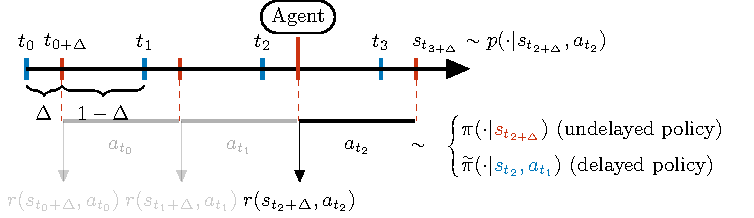
\includegraphics[labelimitation=pendulumvaryingdelay]{img/thesis_plots_imitation.pdf}
    \caption{DIDA 和基线方法在 Pendulum 环境中不同延迟值下的平均回报。
    水平虚线对应无延迟专家（\gls{sac}）的性能。
    阴影区域表示一个标准差，结果基于 10 个种子获得。}
    \label{fig:pendulum_varying_delay_imitation}
\end{figure}

\begin{figure}[t]
    \centering
    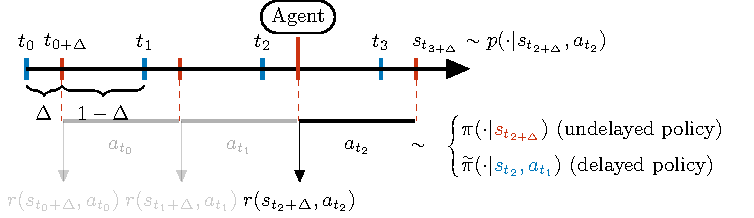
\includegraphics[labelimitation=delay5pendulumimitation]{img/thesis_plots_imitation.pdf}
    \caption{DIDA 和基准方法在 Pendulum 环境中延迟为 5 时获得的回报。
    水平虚线对应专家的回报，垂直虚线表示训练专家所用的步数。
    阴影区域表示一个标准差，结果基于 10 个种子获得。}
    \label{fig:pendulum_imitation}
\end{figure}

\noindent\textbf{随机 Pendulum。}\indent 这些任务的结果如\Cref{fig:noise_pendulum_imitation} 所示。
与前一章相同，噪声按照\Cref{tab:noises} 分为几组。
在左上图中，所有噪声均基于 beta 分布。
在该任务中，DIDA 不仅取得了远优于基线的最终性能，而且收敛到这些性能的速度也远快于基线。
在右上图的第二组中，基线性能接近 DIDA，但 DIDA 仍然显著领先。
最后，在左下图的第三组中，DIDA 再次取得最佳性能。
对于 LogNormal(1.0) 噪声，即使 DIDA 的性能也显著下降，这在意料之中，因为该噪声高度不对称，使信念分布对算法更具挑战性。

\begin{figure}[t]
    \centering
    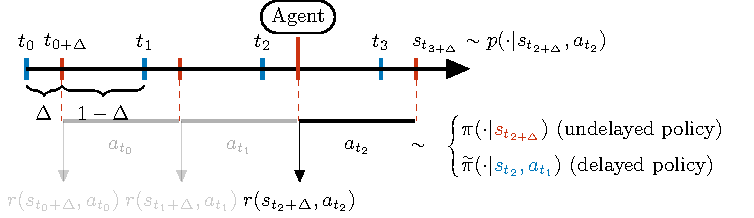
\includegraphics[labelimitation=pendulumnoiseimitation]{img/thesis_plots_imitation.pdf}
    \caption{添加不同噪声（如\Cref{tab:noises} 所述）的 Pendulum 环境中 DIDA 和基线方法获得的回报。
    颜色表示噪声类型，标记表示算法。
    水平虚线表示每种噪声下专家的回报，垂直虚线表示训练专家所用的步数。
    在右上图中，专家性能汇聚在一起。
    阴影区域表示一个标准差，结果基于 10 个种子获得。}
    \label{fig:noise_pendulum_imitation}
\end{figure}

\noindent\textbf{非整数延迟 Pendulum。}\indent 结果如\Cref{fig:pendulum_non_int_imitation} 所示。
在该任务中，DIDA 的性能略低于其在整数延迟上的性能（报告于\Cref{fig:pendulum_varying_delay_imitation}）。
有两个原因。
首先，专家以持久度 2 训练，回报略低。
其次，此处 DIDA 将其动作持续执行 2 步，因此延迟值也翻倍。
\Cref{fig:pendulum_non_int_imitation} 中的延迟 1 对应于\Cref{fig:pendulum_varying_delay_imitation} 中的延迟 2。
无论如何，DIDA 的性能仍然令人满意，表明其能够有效适应非整数延迟。

\begin{figure}[t]
    \centering
    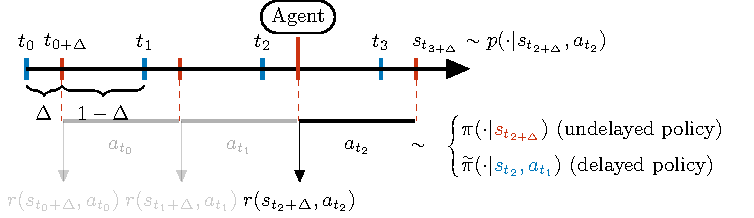
\includegraphics[labelimitation=pendulumnonint]{img/thesis_plots_imitation.pdf}
    \caption{DIDA 在 Pendulum 环境中不同非整数延迟值下的平均回报。
    水平虚线表示无延迟专家（\gls{sac}）的性能。
    阴影区域表示一个标准差，结果基于 10 个种子获得。}
    \label{fig:pendulum_non_int_imitation}
\end{figure}

\noindent\textbf{Mujoco。}\indent 结果如\Cref{fig:mujoco_imitation} 所示。
此处再次，DIDA 和 M-DIDA 取得了相似性能，同时优于所有基线。
部分由于延迟的初始化偏移，在 HalfCheetah 和 Reacher 中，DIDA 的表现远差于无延迟专家。
更令人惊讶的是，在 Swimmer 中，DIDA 的表现略好于专家。
这是延迟初始化偏移的一个意外后果。
事实上，在某些环境中，初始随机动作序列可能将智能体置于有利状态。
在 HalfCheetah 中，随机动作有时使智能体头朝下，因此必须先站起来才能移动。而在 Swimmer 中，随机动作为智能体提供了初始速度。

\begin{figure}[t]
    \centering
    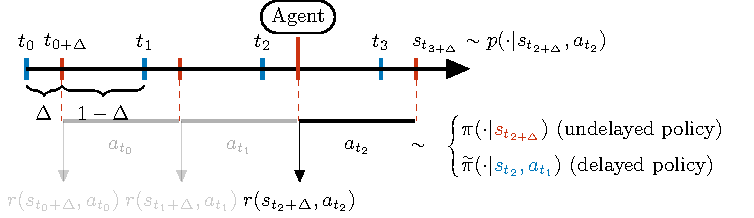
\includegraphics[labelimitation=delay5mujocoimitation]{img/thesis_plots_imitation.pdf}
    \caption{DIDA 和基准方法在各种 Mujoco 环境中获得的回报。
    水平虚线对应专家的回报，垂直虚线表示训练专家所用的步数。
    阴影区域表示一个标准差，结果基于 10 个种子获得。}
    \label{fig:mujoco_imitation}
\end{figure}

\noindent\textbf{Trading。}\indent 对于该任务，报告训练集（2019）上获得的结果，如\Cref{fig:trading_dida} 所示。
鉴于买卖价差的存在对回报具有决定性影响，仅获得正回报便已是不小的成就。
DIDA 不仅取得了正回报，而且明显优于延迟专家。
令人惊讶的一点是，DIDA 初始时获得了比专家本身更好的回报。
策略实际上略有不同。
在\Cref{fig:allocation} 中，通过表示 DIDA 学习到的策略与专家策略的动作模式对比，分析 DIDA 学习到的策略。
具体来说，该图说明了批量 RL 设定的困难。
DIDA 在第 10 次迭代学习到的策略与训练集上的专家非常相似，但开始偏离测试集上的专家。

\begin{figure}[t]
    \centering
    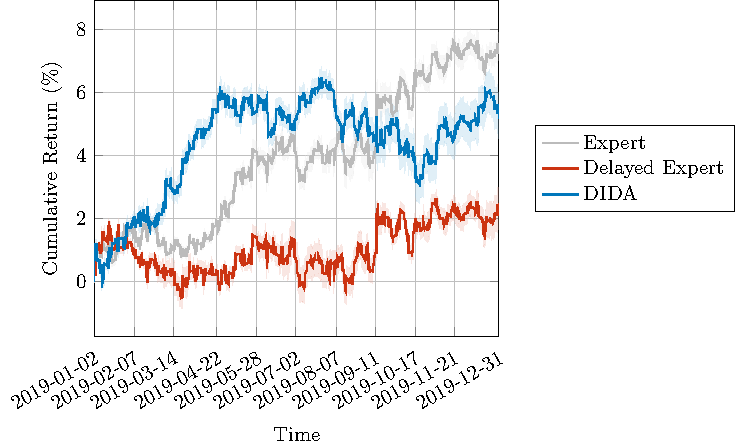
\includegraphics[labelimitationtrading=didatradingeurusd]{img/thesis_plots_chapter_imitation_trading.pdf}
    \caption{2019 年 EUR-USD 货币对交易的累计回报（占投资金额的百分比）。
    DIDA 与其训练的专家以及一个超参数在延迟数据集上选择的无延迟专家（称为"延迟专家"）进行比较。}
    \label{fig:trading_dida}
\end{figure}


\begin{figure*}[t]
\centering
    \begin{subfigure}{0.33\textwidth}
        \centering
        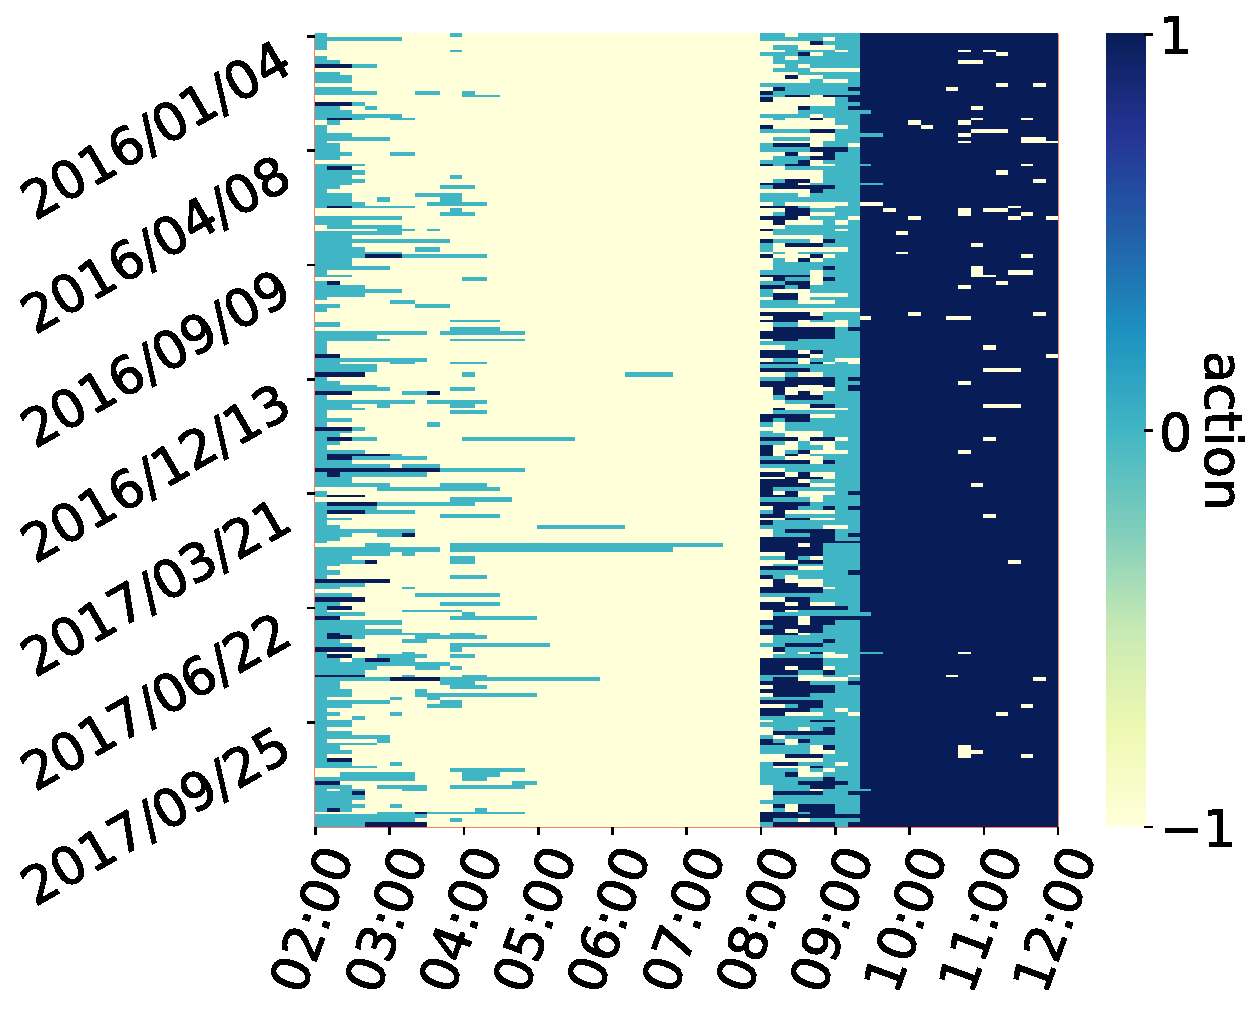
\includegraphics[width=\linewidth]{img/imitation/expert_2016_2017_regular_shift50_expite_10_expseed_0_allocations.pdf}
        \caption{专家，2016-2017。}
        \label{fig:test_expert_fx_allocation}
    \end{subfigure}%
\hfill
    \begin{subfigure}{0.33\textwidth}
        \centering
        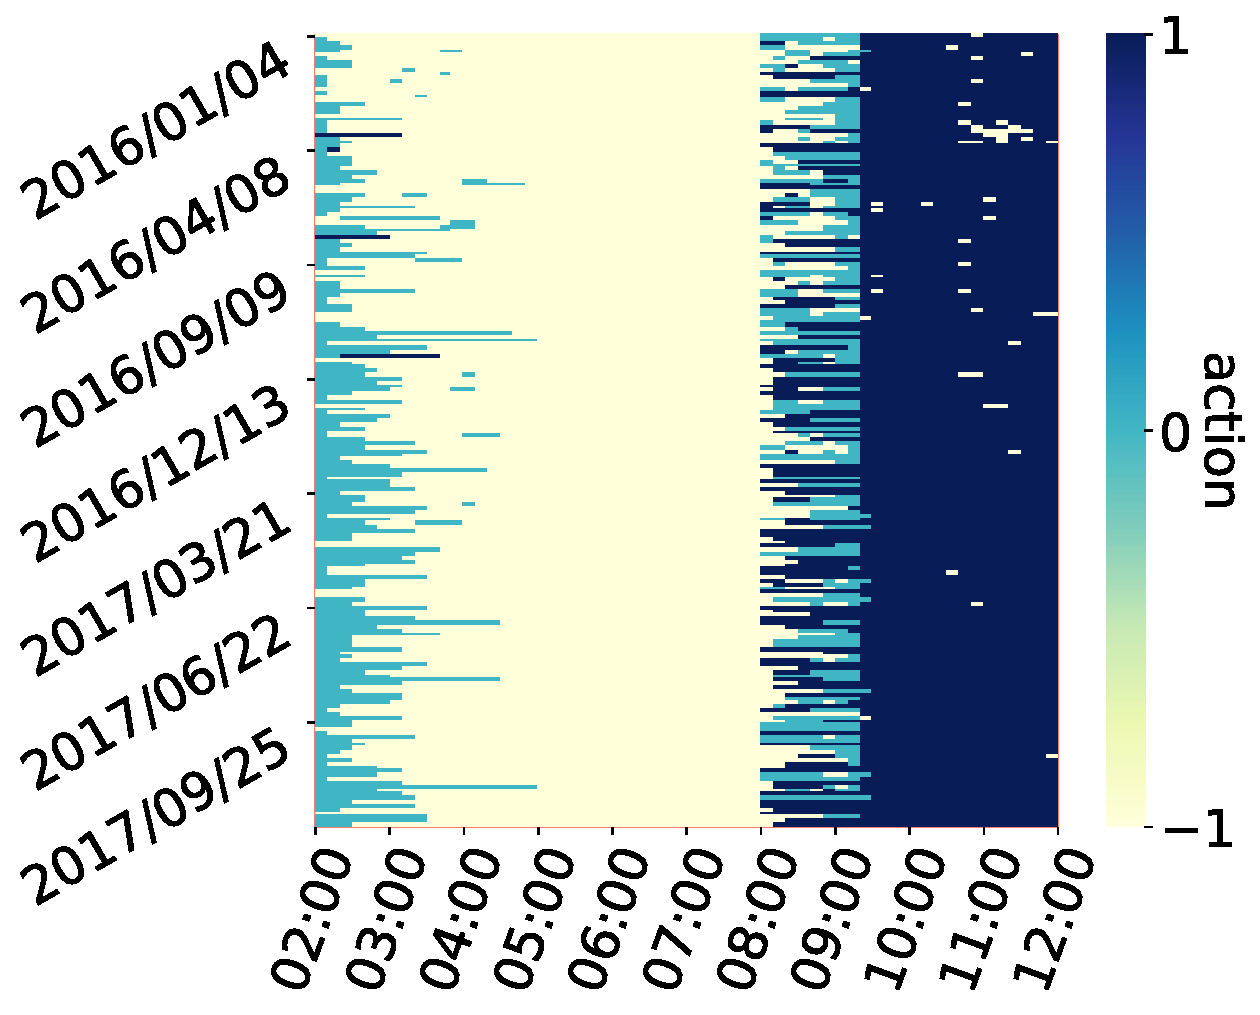
\includegraphics[width=\linewidth]{img/imitation/dida_ms100_est100_shift50_2016_2017_expite_10_expseed_0_dagite_10_dagseed1_allocations.pdf}
        \caption{DIDA，2016-2017。}
        \label{fig:train_dida_fx_allocation}
    \end{subfigure}%
    \begin{subfigure}{0.33\textwidth}
        \centering
        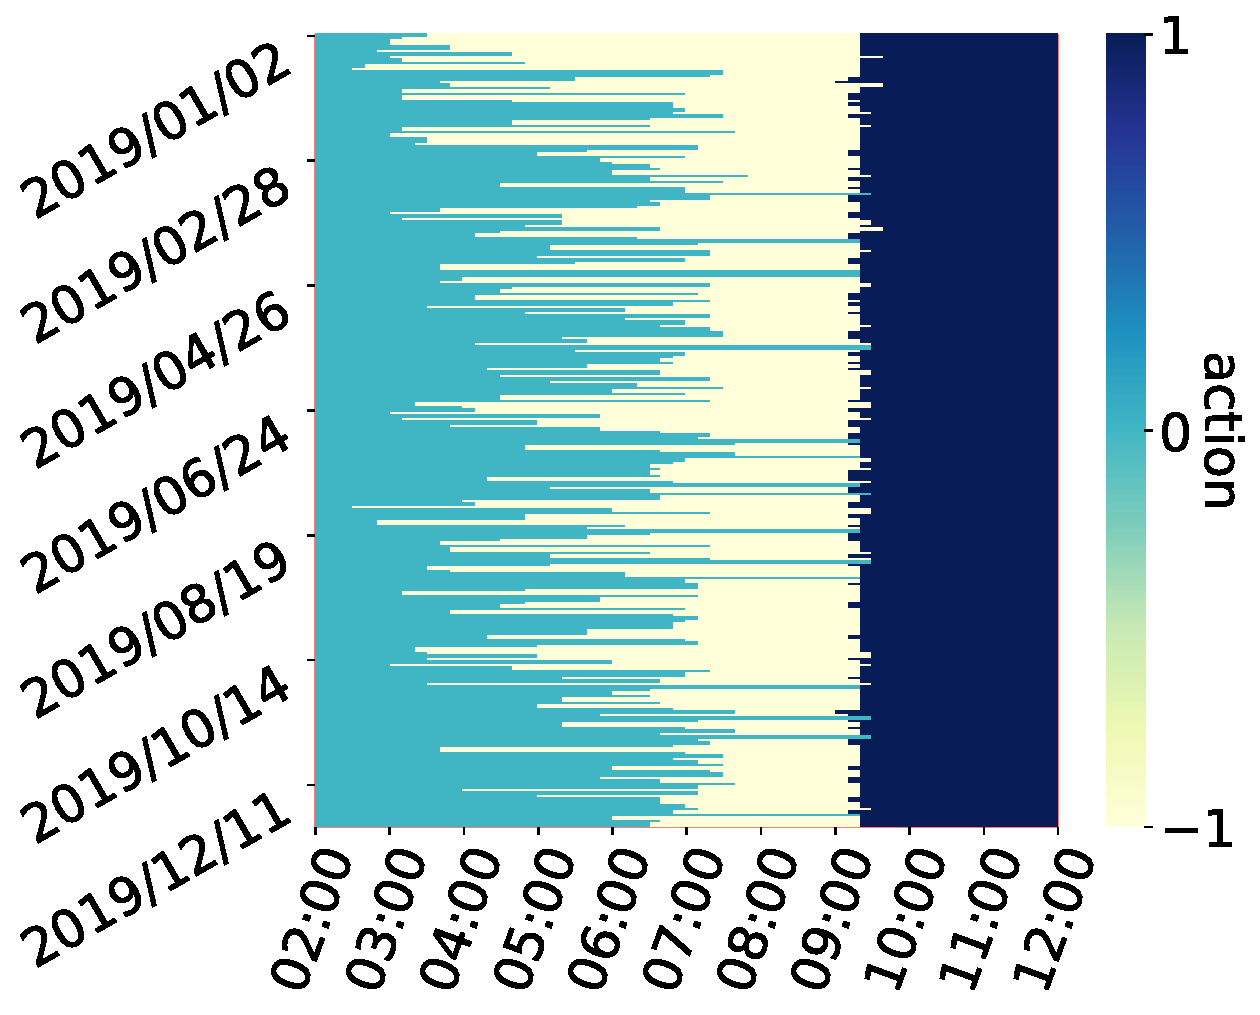
\includegraphics[width=\linewidth]{img/imitation/dida_ms100_est100_shift50_2019_expite_10_expseed_0_dagite_10_dagseed1_allocations.pdf}
        \caption{DIDA，2019。}
        \label{fig:test_dida_fx_allocation}
    \end{subfigure}%
\caption{表示 Trading 任务中专家的动作模式和 DIDA 的动作模式的热力图。
将专家的动作模式（左）与 DIDA 在第 10 次迭代的动作模式进行比较，分别在训练集（2016-2017，中）和测试集（2019，右）上。
热力图显示给定天（行）的给定分钟（列）所选的动作（颜色）。}
\label{fig:allocation}
\end{figure*}

\noindent\textbf{同时学习多重延迟。}\indent 此处探索\Cref{subsubsec:multi_delay_once_imitation} 中提出的思路，即将 DIDA 针对某个延迟 $\delay>0$ 学习的策略应用于更小的延迟 $0<\delay'<\delay$。
在\Cref{fig:pendulum_multi_delay_imitation} 中，给出 Pendulum 任务的结果，其中 DIDA 策略在延迟 $\delay=10$ 上训练。
在\Cref{fig:mujoco_multi_delay_imitation} 中，给出 mujoco 任务的结果，其中 DIDA 策略在延迟 $\delay=5$ 上训练。
显然且符合预期，在较小延迟上获得的性能与 DIDA 在训练所用延迟上达到的性能相似。



\begin{figure}[t]
    \centering
    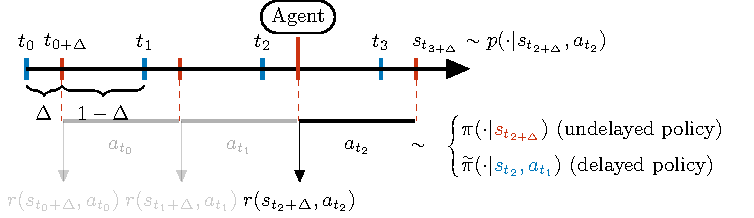
\includegraphics[labelimitation=multipledelayspendulumimitation]{img/thesis_plots_imitation.pdf}
    \caption{在 Pendulum 上，以延迟 10 训练的 DIDA 在较小延迟上测试获得的回报。}
    \label{fig:pendulum_multi_delay_imitation}
\end{figure}

\begin{figure}[t]
    \centering
    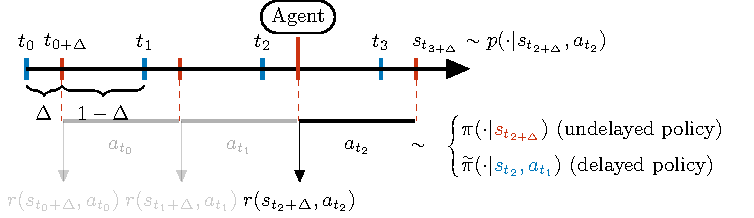
\includegraphics[labelimitation=multipledelaysmujocoimitation]{img/thesis_plots_imitation.pdf}
    \caption{在多种 Mujoco 环境中，以延迟 5 训练的 DIDA 在较小延迟上测试获得的回报。}
    \label{fig:mujoco_multi_delay_imitation}
\end{figure}
